\chapter{Design}
\label{Design}

As we specified the requirements, we can go further into the design part of the system, and that is what we are going to explain in this chapter. 
First of all, we will define the protocol of the system. Moreover, secondly, we will describe the client- and server- sides of it.

\section{Overview of the protocol}

The fundamental part of the WebCache will be its protocol design. We need to examine the following cases, in order to specify the protocol of the application:

    \begin{itemize}
        \item {A client receives an update from the server}
        \item {A client sends an update to the server}
        \item {Two clients interact with a server}
    \end{itemize}

\subsection{The way of exchaning the data}

Because the AntidoteDB is using CRDT datatypes, the following options are possible to update the database: state-based and operation-based. Due to the time constraints and the amount of work, this thesis will consider only the operation-based approach, which was described in the theoretical background chapter. Therefore, whenever a client wants to update the database, it will send to the server a list of operations. However, whenever it wants to read the value, it will receive the current state of the object from the database.

For this thesis, we are going to use such datatypes as counters and sets. As was already mentioned in the Introduction chapter, the counter is a number datatype, which allows incrementing and decrementing the value. Reading a counter will return the aggregated value of all performed operations. 



\subsection{A client receives an update from the server}

Let us say that a client requests an update from the server. In this case, if the request is successful, the server is going to respond with a value for the requested key and the timestamp of the last write -- \textit{t\textsubscript{0}}.

\begin{figure}[!htb]
    \setlength{\fboxsep}{4pt}%
    \setlength{\fboxrule}{1pt}%
    \fbox{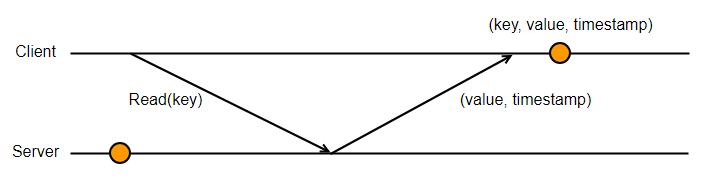
\includegraphics[width=\linewidth]{images/architecture/read1.png}}
    \caption{The way a client receives a key-value update from the server.}
    \label{fig:design2}
\end{figure}

In case a client receives an update from the server, and that update has an earlier timestamp than the one, which is already stored in the client's cache, then a client skips it and can try later for fresher updates. The implementation of this will be explained later in the chapter of implementation.

\subsection{A client sends an update to the server}

In the case of writing the information to the server, a client has to send a key with an operation to the server. Then the acknowledgment with a timestamp is going to be sent back to the client.

\begin{figure}[!htb]
    \setlength{\fboxsep}{4pt}%
    \setlength{\fboxrule}{1pt}%
    \fbox{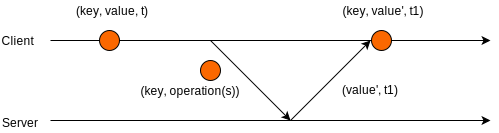
\includegraphics[width=\linewidth]{images/architecture/write.png}}
    \caption{The way a client sends a write operation to the server.}
    \label{fig:design3}
\end{figure}

\subsection*{Several updates on a client while offline}

The client is capable of performing updates when offline. These updates will take effect immediately. However, in order for them to be applied to the server, the client has to be back online. Once the connection is established again, all the updates that were performed on the client-side in offline mode will be sent to the server.

\subsection{Two clients interact with a server.}

\begin{figure}[!htb]
    \setlength{\fboxsep}{4pt}%
    \setlength{\fboxrule}{1pt}%
    \fbox{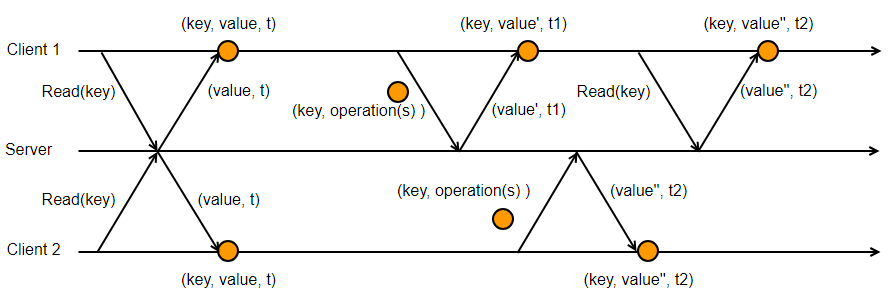
\includegraphics[width=\linewidth]{images/architecture/twoclients.png}}
    \caption{Graphical representation over a possible communicaton between two clients and a server.}
    \label{fig:design4}
\end{figure}

Let us assume that initially, the server has the key-value pair \textit{(k, v)} at the timestamp \textit{t\textsubscript{0}}. Therefore, after both clients receive updates from the server, they consist of the \textit{(k, v)} pair at the timestamp \textit{t\textsubscript{0}}. In case clients change the value under mentioned key to something else, they will have to get an acknowledgement from the server in order to receive a unique timestamp related to the change. At the representation above, a \textit{Client 1} is acting first and getting an acknowledgement of its change at the time \textit{t\textsubscript{1}}, while Client \textit{Client 2} makes the change later at time \textit{t\textsubscript{2}}. That makes \textit{Client 1} receive a new value \textit{v''}, when it reads the information from the server again.

\section{System's main components}


As the protocol is explained, we can start designing the system. Let us have a look at the main components of it:

\begin{figure}[!htb]
    \begin{center}
    \setlength{\fboxsep}{4pt}%
    \setlength{\fboxrule}{1pt}%
    \fbox{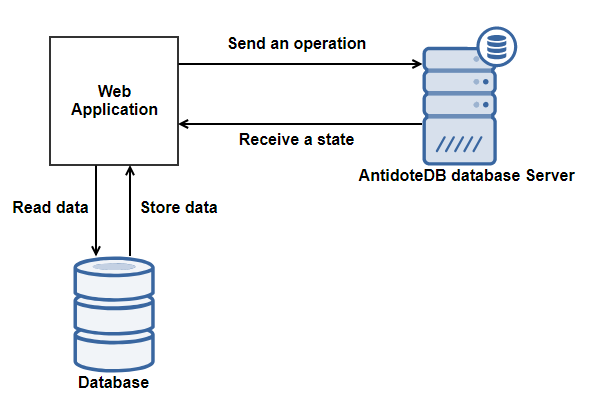
\includegraphics[width=\linewidth]{images/design/diagram2.png}}%
    \caption {An overview of the system's design.}
    \label{fig:design5}
\end{center}
\end{figure}

\subsection{Web Application}

First of all, in order for the user to be able to communicate with an AntidoteDB server, we are going to have a running web application that serves as a client. It runs in the web-browser, supports various commands from the user and sits on top of the local database layer. 

\vspace{5mm}These are the supported commands:

\begin{itemize}
    \item \textit{read(key)} -- an asynchronous function that pulls database changes concerning the \textit{key} that the user passed.
    \item \textit{update(key, op)}  -- an asynchronous function that processes user-made updates.
     \begin{itemize}
         \item \textit{key}: a key, which is going to be updated;
         \item \textit{op}: an operation, which is going to be performed on the key;
     \end{itemize}
  \end{itemize}

\subsection{Server}

It is a configured AntidoteDB server that supports the following scenarios:

\begin{itemize}
    \item receiving an operations or an array of operations performed on a CRDT-object, according to the key, and applying them on the server;
    \item sending back to the client the state of requested CRDT-object / objects according to their state on the server;
    %\item sending back states of all stored CRDT-objects, if a specific object was not asked for; 
\end{itemize}

\subsection{A database layer}

This layer should consist of the database, which is going to store the actual states of CRDT-objects, as well as user-added operations performed on the states.
When a user performs \textit{read} by \textit{key} operation from the cache, the following actions are taking place:

\begin{itemize}
\item Firstly, the state of the object \textit{\textbf{O}} is going to be found by \textit{\textbf{key}} in the database
\item Next, operations \textit{\textbf{o}} performed on the object \textit{\textbf{O}} are selected
\item Afterwards, selected operations \textit{\textbf{o}} applied on the object \textit{\textbf{O}}.
\item Finally, the object from the previous step is returned back as a response to the application.
\end{itemize} 

\section{Offline functionality}

In this section, we are going to describe the offline functionality of the system.

Initially, the database is empty. Therefore, if the user is offline from the very beginning, he should be able to add the data into the database himself. 
The system represented in \textbf{Figure \ref{fig:design5}} will change by having only the Web Application and the database. However, whenever the connection is established with the server, the operations, which were stored in local database while offline, will be sent to the server. 

At the \textbf{Figure \ref{fig:design6}}, the sequence of getting the data from the local database is shown. This case describes the scenario, when the server is unavailable and the application continues its work in an offline mode.
 
\begin{figure}[!htb]
    \begin{center}
    \def\svgwidth{\columnwidth}
    \input{images/design/offlineProtocol.pdf_tex}
    \caption {Successful request of state from the local database -- Sequence diagram.}
    \label{fig:design6}
\end{center}
\end{figure}

\begin{figure}[!htb]
    \begin{center}
    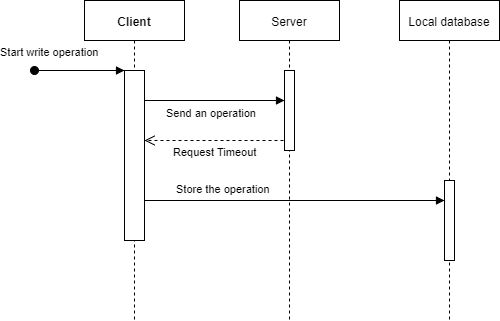
\includegraphics[width=\linewidth]{images/design/offlineProtocol_send.png}%
    \caption {Successful storing of an operation in the local database -- Sequence diagram.}
    \label{fig:design7}
\end{center}
\end{figure}

At the \textbf{Figure \ref{fig:design7}}, the sequence of storing the data locally is shown. This case describes the scenario, when the server is unavailable and the application continues its work in an offline mode.


\section {Online functionality}

In this section, we are going to describe the online functionality of the system.



\section {The transition between offline and online modes}